% ==============================================================================
% PG - Sophie Dilhon
% Capítulo 4 - Projeto Arquitetural e Implementação
% ==============================================================================
\chapter{Projeto Arquitetural e Implementação}
\label{chap-projeto}

\section{Modelos FrameWeb}
\label{sec-projeto-frameweb}

Nessa seção são apresentados os modelos FrameWeb, construídos na fase de Projeto Arquitetural
do SCAP, com o objetivo de guiar a fase de implementação do sistema.

\subsection{Modelo de Entidades}
\label{subsec-frameweb-entidades}
O modelo de entidades de FrameWeb é um diagrama de classes UML que representam
os objetos de domínio do problema e seu mapeamento para a persistência no banco de dados
relacional. A partir dele são implementadas as classes da camada de domínio~\cite{souza:2007}.

A Figura \ref{fig-modelo-entidades} apresenta o modelo de entidades do SCAP. O modelo foi feito
a partir do diagrama de classes mostrado anteriormente, com adaptações para a plataforma 
escolhida para a implementação do sistema, dessa forma são apresentados os tipos
de cada propriedade. A Figura \ref{fig-modelo-entidades-enum} apresenta
os tipos enumerados do modelo de entidades do SCAP.

\sophie{Adicionar null}
\begin{figure}
    \centering
    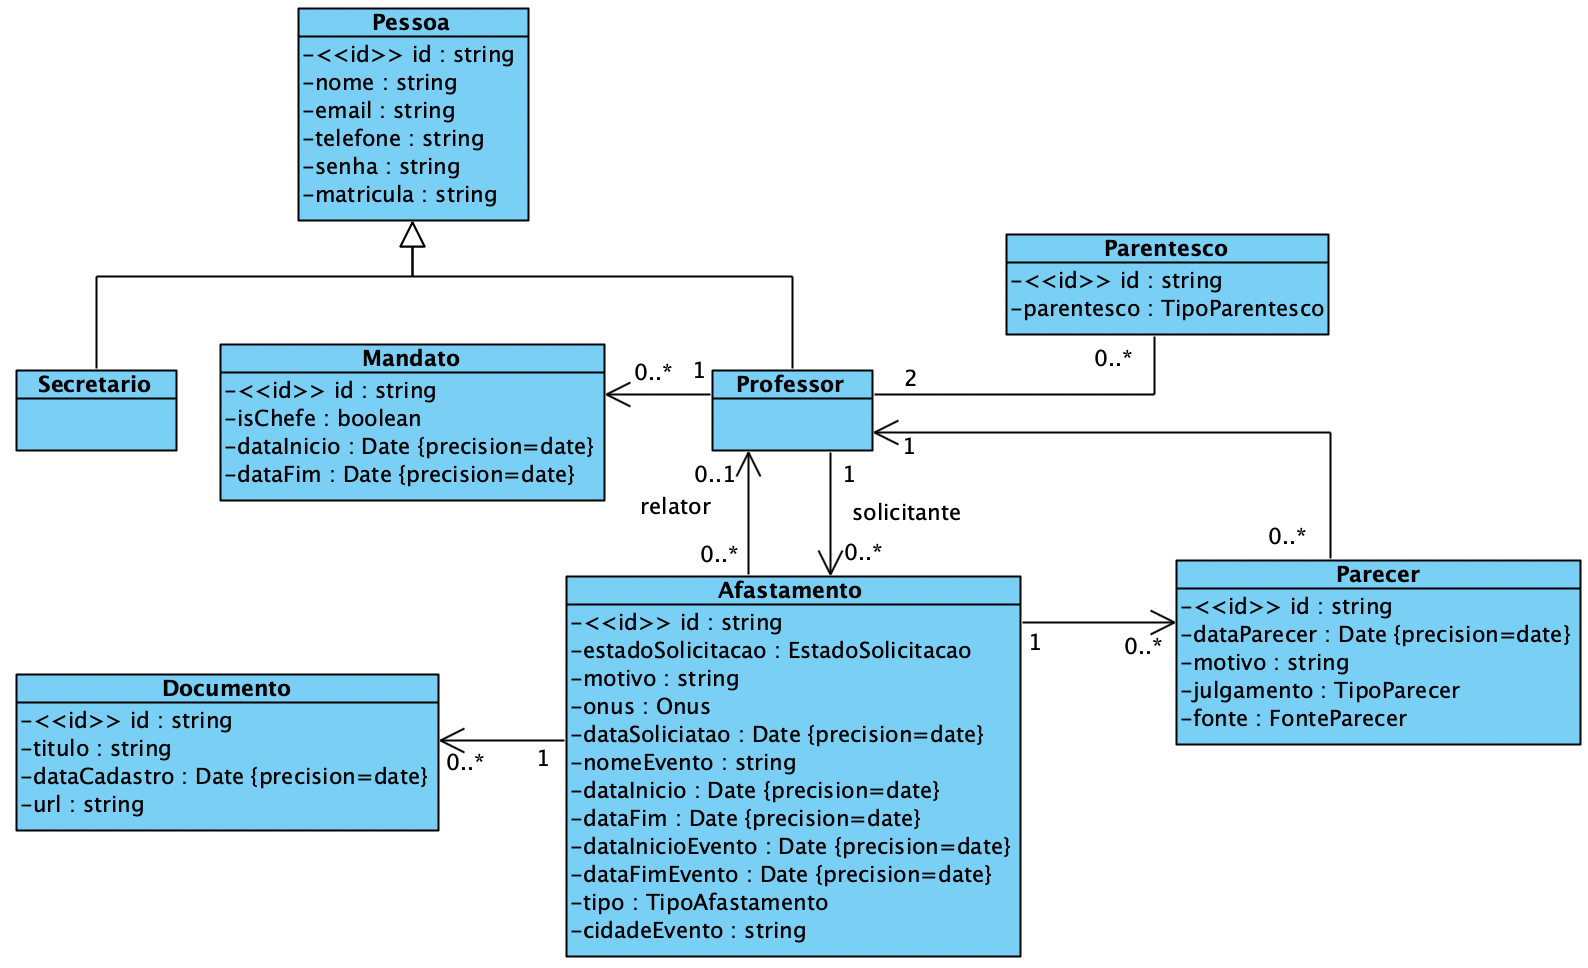
\includegraphics[width=1\textwidth]{figuras/fig-modelo-entidades.png}
    \caption{Modelo de Entidades do SCAP.}
    \label{fig-modelo-entidades}
\end{figure}

\begin{figure}
    \centering
    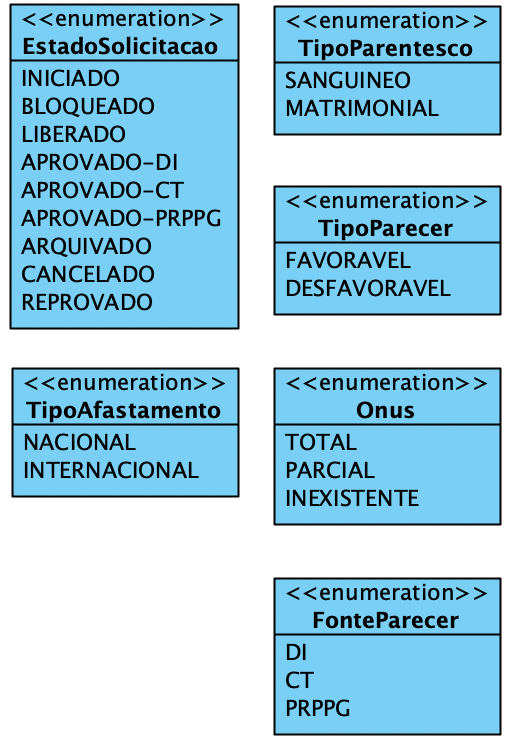
\includegraphics[width=0.5\textwidth]{figuras/fig-modelo-entidades-enum.png}
    \caption{Tipos Enumerados do Modelo de Entidades do SCAP.}
    \label{fig-modelo-entidades-enum}
\end{figure}


\subsection{Modelo de Persistência}
\label{subsec-frameweb-persistencia}

O modelo de persistência de FrameWeb é um diagrama de classes UML que representa
as classes responsáveis pela persistência das classes de domínio no banco de dados~\cite{souza:2007}.
Foi utilizado o padrão \textit{Repository} para a implementação das classes de persistência,
este propõe uma camada de separação entre o domínio e o mapeamento de dados.

\sophie{Acho que o get com filtros pode ser do IBase mas não ser definido em BaseRepository (filtros vão ser específicos de cada entidade)}


Para isso, foi criada uma interface base (\textbf{IBase}) que define os métodos comuns a todas as classes de persistência,
sendo eles: \textit{get} para buscar todos os elementos com base nos filtros passados como parâmetro,
\textit{post} para criar um novo elemento, \textit{getById} para buscar um elemento a partir de seu
\textit{id} e \textit{delete}. A Figura \ref{fig-modelo-persist-base} apresenta essa interface e a
classe \textit{Repository} que a implementa. O tipo genérico \textit{T} representa a classe de domínio
sendo manipulada, ou seja, em \textbf{AfastamentoRepository} o método \textit{getById}
retorna um elemento da classe \textbf{Afastamento}.


\begin{figure}[h!]
    \centering
    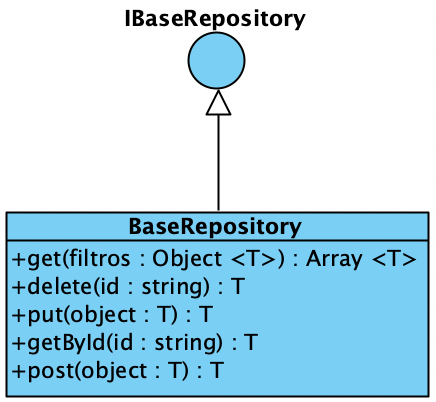
\includegraphics[width=0.4\textwidth]{figuras/fig-modelo-persist-base.png}
    \caption{Interface e Implementação do Repository Base.}
    \label{fig-modelo-persist-base}
\end{figure}


As interfaces do modelo herdam \textbf{IBase}, enquanto as classes \textit{Repository} estendem a
classe \textbf{BaseRepository}. De modo que todas as classes de persistência possuam, além dos métodos
específicos dessas, os métodos comuns definidos na interface base. As Figuras \ref{fig-modelo-persist}
apresentam o modelo de persistência do SCAP.

\begin{figure}[h!]
    \centering
    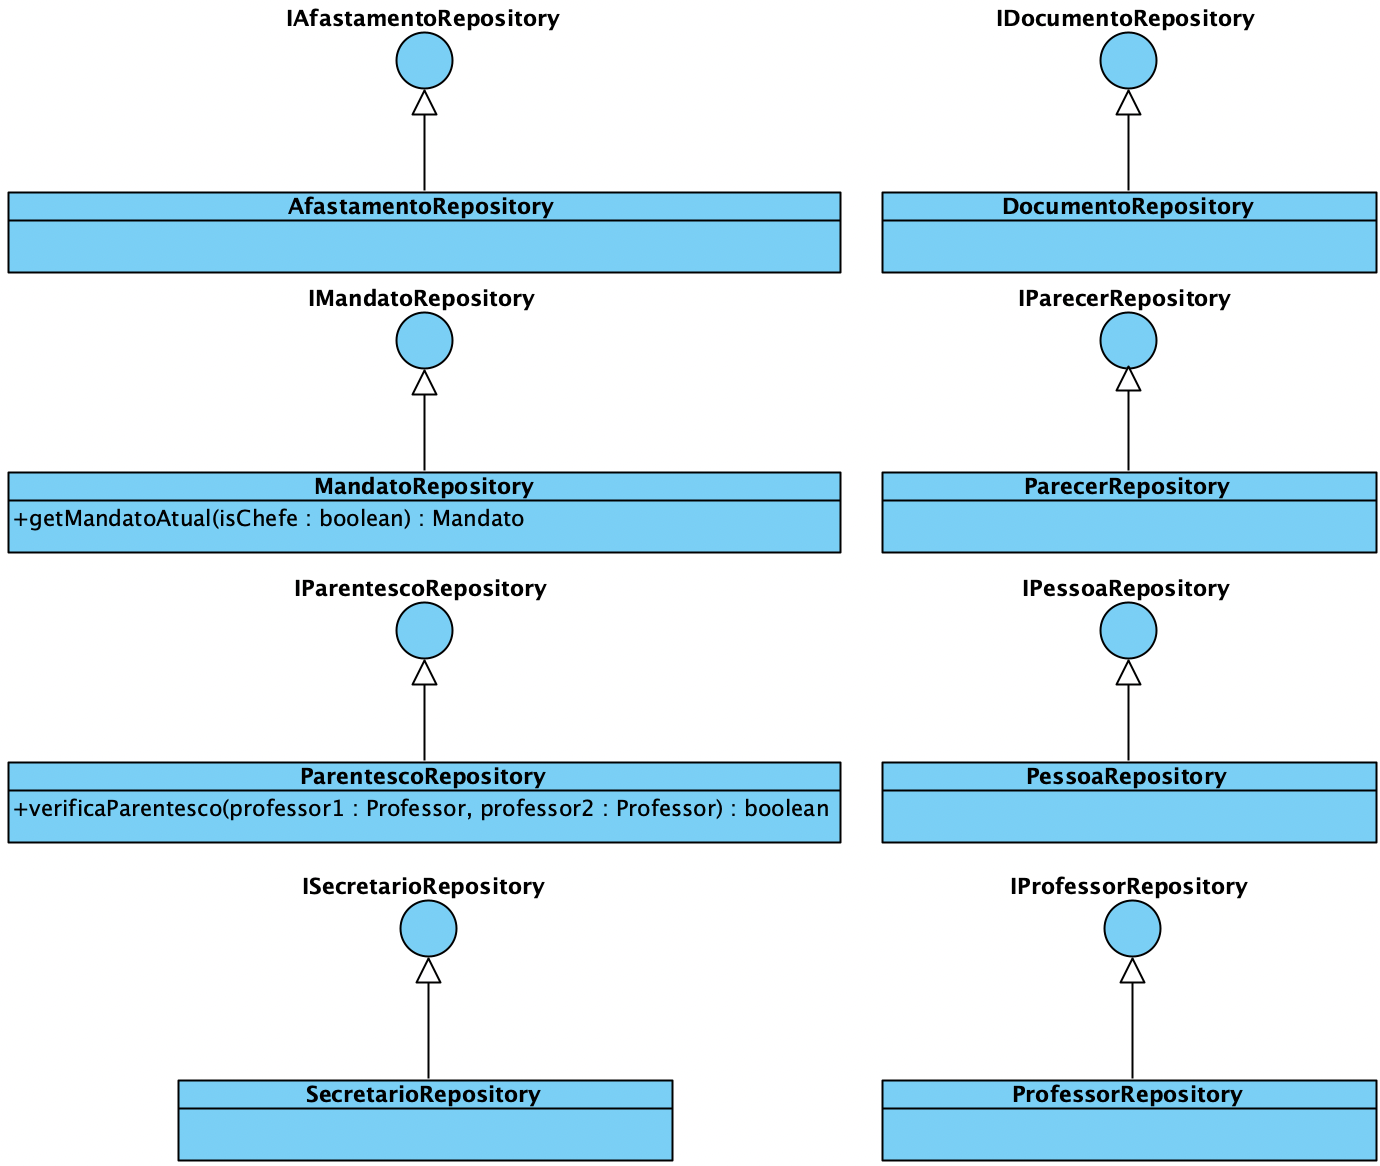
\includegraphics[width=0.9\textwidth]{figuras/fig-modelo-persist.png}
    \caption{Modelo de Persistência do SCAP.}
    \label{fig-modelo-persist}
\end{figure}


\subsection{Modelo de Navegação}
\label{subsec-frameweb-navegacao}

O Modelo de Navegação é um diagrama de classe da UML que representa os diferentes componentes que
formam a camada de Lógica de Apresentação, como páginas Web, formulários HTML e classes de ação do framework específico~\cite{souza:2007}. 
Esse modelo é utilizado para guiar a implementação dos pacotes Visão e Controle.

A Tabela \ref{tab-estereotipos-navegacao} apresenta os estereótipos UML utilizados no modelo de navegação do SCAP,
propostos por~\citeonline{hoppe:2023} como uma adaptação, para \textit{frameworks} SPA,
dos estereótipos propostos originalmente por~\citeonline{souza:2007}.

\begin{table}[h!]
    \centering
    \caption{Estereótipos UML para Modelos de Navegação~\cite{hoppe:2023}.}
    \label{tab-estereotipos-navegacao}
    \begin{tabular}{|p{3cm}|p{12cm}|}
        \hline
        \textbf{Estereótipo} & \textbf{Descrição} \\
        \hline
        (Nenhum)    & Controladora de um framework Front Controller ou a parte controladora de um component de um framework SPA. \\
        \hline
        <<Page>>    & Página Web estática ou dinâmica. \\
        \hline
        <<Partial>> & Parte de uma página HTML que é gerada em tempo de execução por meio de AJAX. \\
        \hline
        <<Form>>    & Formulário HTML \\
        \hline
    \end{tabular}
\end{table}

A Figura \ref{fig-modelo-navegacao-afast} apresenta o modelo de navegação do SCAP para os casos de uso
\textbf{Cancelar Afastamento}, \textbf{Cadastrar Afastamento} e \textbf{Consultar Afastamento}.

\begin{figure}
    \centering
    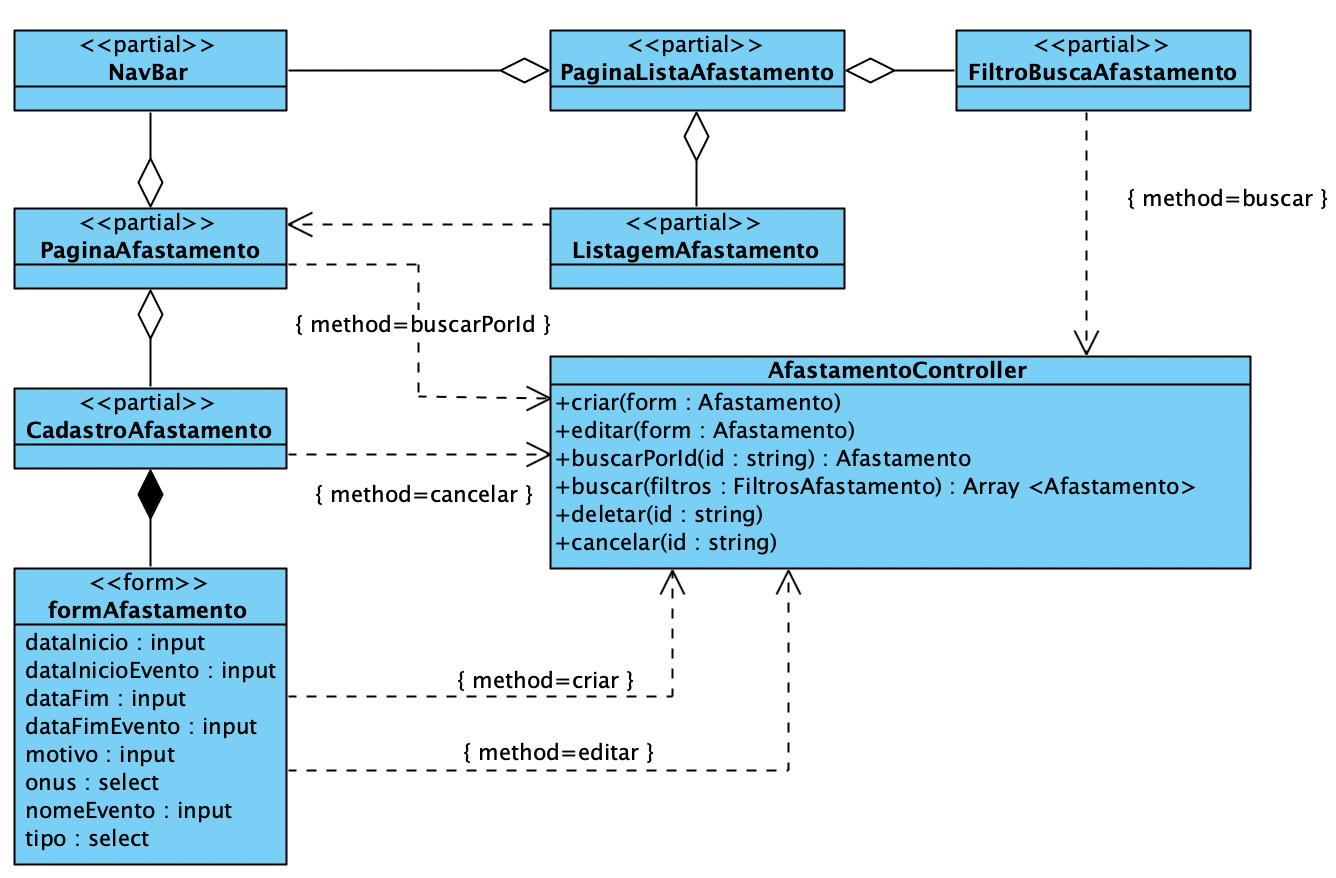
\includegraphics[width=1\textwidth]{figuras/fig-modelo-naveg-afast.png}
    \caption{Modelo de Navegação do SCAP.}
    \label{fig-modelo-navegacao-afast}
\end{figure}

A \textbf{PaginaListaAfastamento} é responsável por listar os afastamentos cadastrados.
Ela possui um componente filtro (\textbf{FiltroBuscaAfastamento}), em que é possível buscar
os afastamentos por diferentes critérios, definidos pela interface mostrada na Figura \ref{fig-interface-filtro-afast}.
O componente \textbf{ListagemAfastamento} consiste de uma tabela que lista os afastamentos buscados,
cada linha da tabela possui um botão que redireciona para a página de detalhes do afastamento (\textbf{PaginaAfastamento}).

\begin{figure}
    \centering
    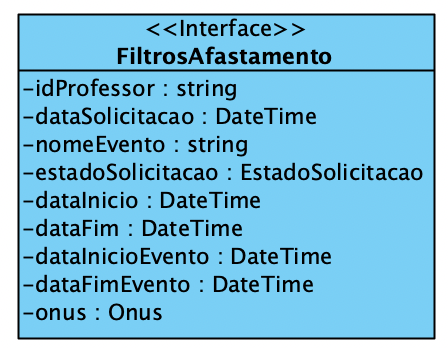
\includegraphics[width=0.5\textwidth]{figuras/fig-interface-filtro-afast.png}
    \caption{Interface Filtro Afastamento.}
    \label{fig-interface-filtro-afast}
\end{figure}

Se redirecionado para a \textbf{PaginaAfastamento} a partir do componente \textbf{ListagemAfastamento},
o \textit{partial} possui o atributo \textbf{id} inicializado com o \textit{id} do afastamento, e é
utilizado para fazer uma chamada ao método \textbf{buscarPorId} da \textit{controller} \textbf{AfastamentoController}.
Caso o usuário seja o solicitante do afastamento, ele pode cancelá-lo clicando em um botão que faz uma chamada ao método
\textbf{cancelar} da \textit{controller} \textbf{AfastamentoController}.

Quando não possui um \textit{id} inicializado, o \textit{partial} é utilizado para criar um novo afastamento,
o usuário deve então preencher os campos do formulário e clicar em um botão que faz uma chamada ao método
\textbf{criar} da \textit{controller} \textbf{AfastamentoController}.


\begin{figure}
    \centering
    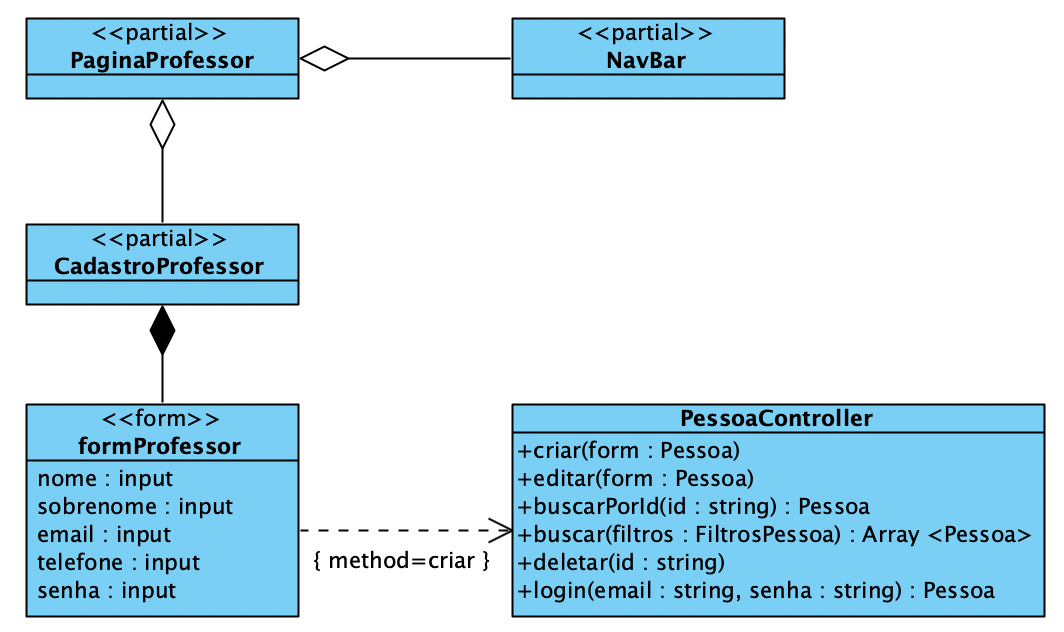
\includegraphics[width=0.9\textwidth]{figuras/fig-modelo-naveg-cadast.png}
    \caption{Modelo de Navegação do SCAP do Caso de Uso Cadastrar Professor.}
    \label{fig-modelo-navegacao-professor}
\end{figure}

A Figura \ref{fig-modelo-navegacao-professor} apresenta o modelo de navegação do SCAP para o caso de uso
\textbf{Cadastrar Professor}. Na \textbf{PaginaProfessor} o secretário pode cadastrar um novo professor,
para isso ele deve preencher os campos do formulário e clicar em um botão que faz uma chamada ao método
\textbf{criar} da \textit{controller} \textbf{PessoaController}.


\subsection{Modelo de Aplicação}
\label{subsec-frameweb-aplicacao}
O Modelo de Aplicação é um diagrama de classes da UML que representa as classes de
serviço, que são responsáveis pela codificação dos casos de uso, e suas dependências~\cite{souza:2007}.
Por ele pode-se visualizar a dependência entre os pacotes Controle (classes de ação),
Aplicação (classes de serviço) e Persistência (interfaces \textit{Repository}). 

As Figuras \ref{fig-modelo-aplicacao-1} e \ref{fig-modelo-aplicacao-2} contém os Modelos de Aplicação.
As solicitações dos usuários são tratadas pelas classes de controle, que por sua vez
chamam as classes de serviço para realizar as operações de negócio, que por fim acessam
as classes de persistência para realizar as operações de leitura e escrita no banco de dados.


\begin{figure}[h!]
    \centering
    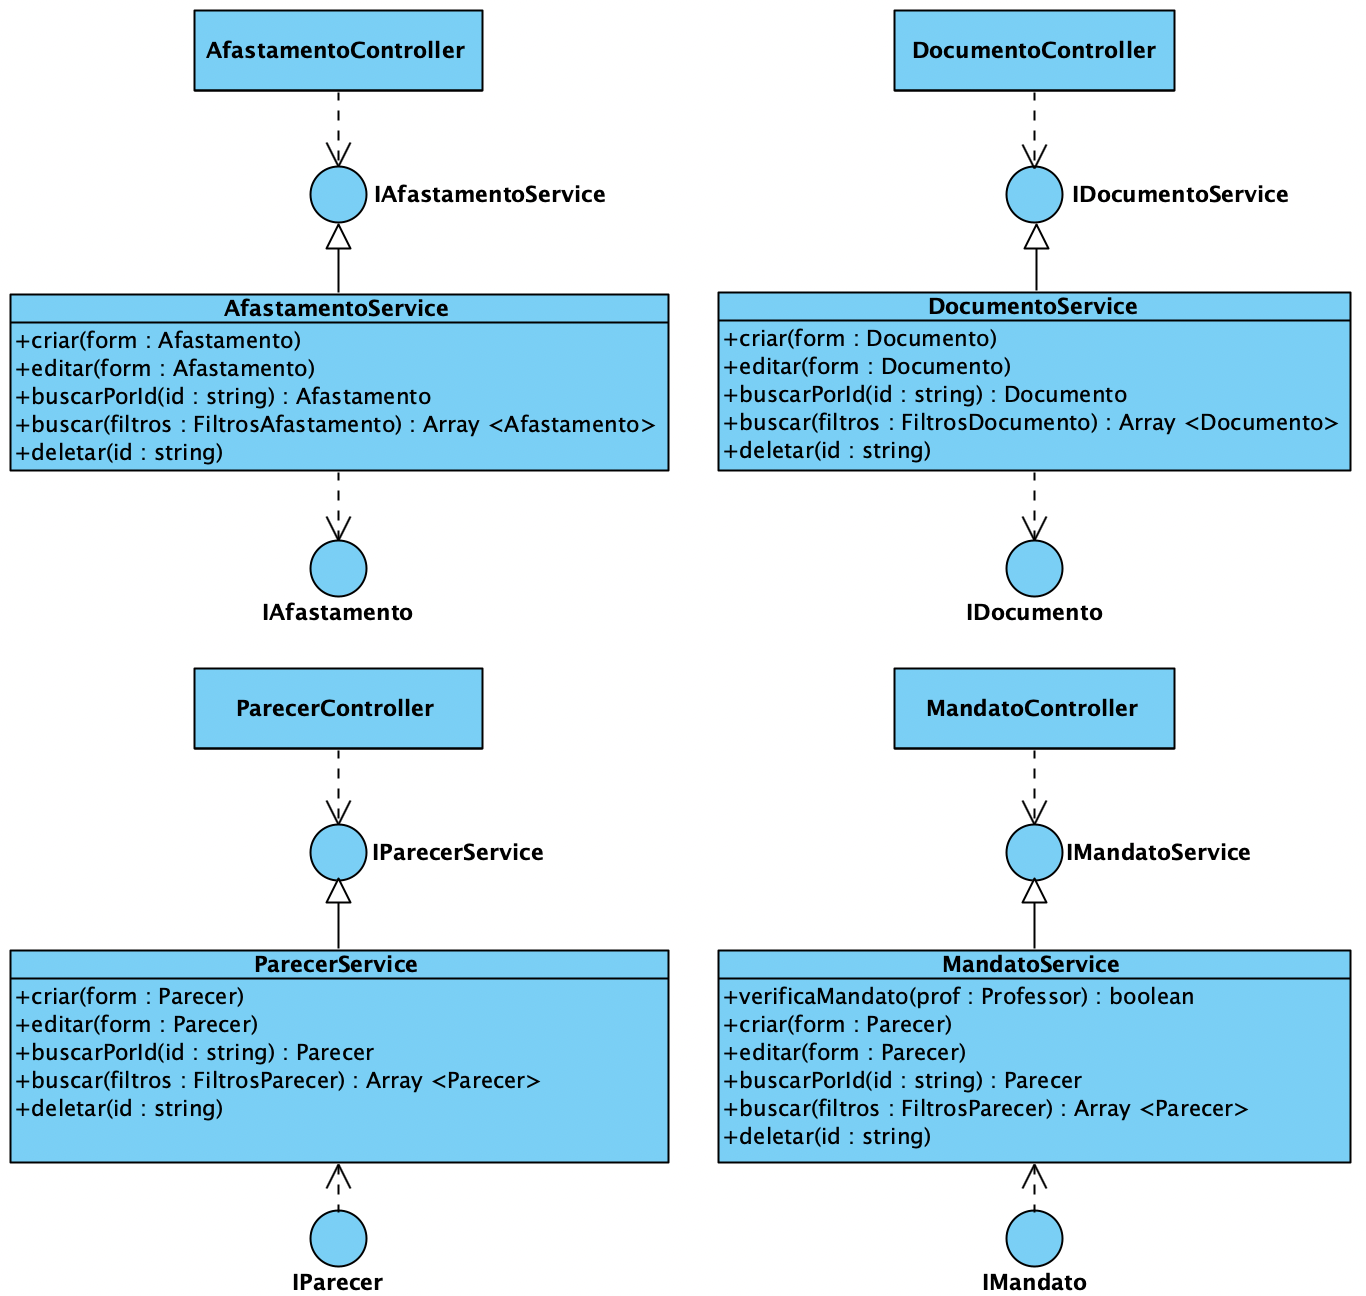
\includegraphics[width=0.9\textwidth]{figuras/fig-modelo-apl-1.png}
    \caption{Modelo de Aplicação do SCAP.}
    \label{fig-modelo-aplicacao-1}
\end{figure}

\begin{figure}[h!]
    \centering
    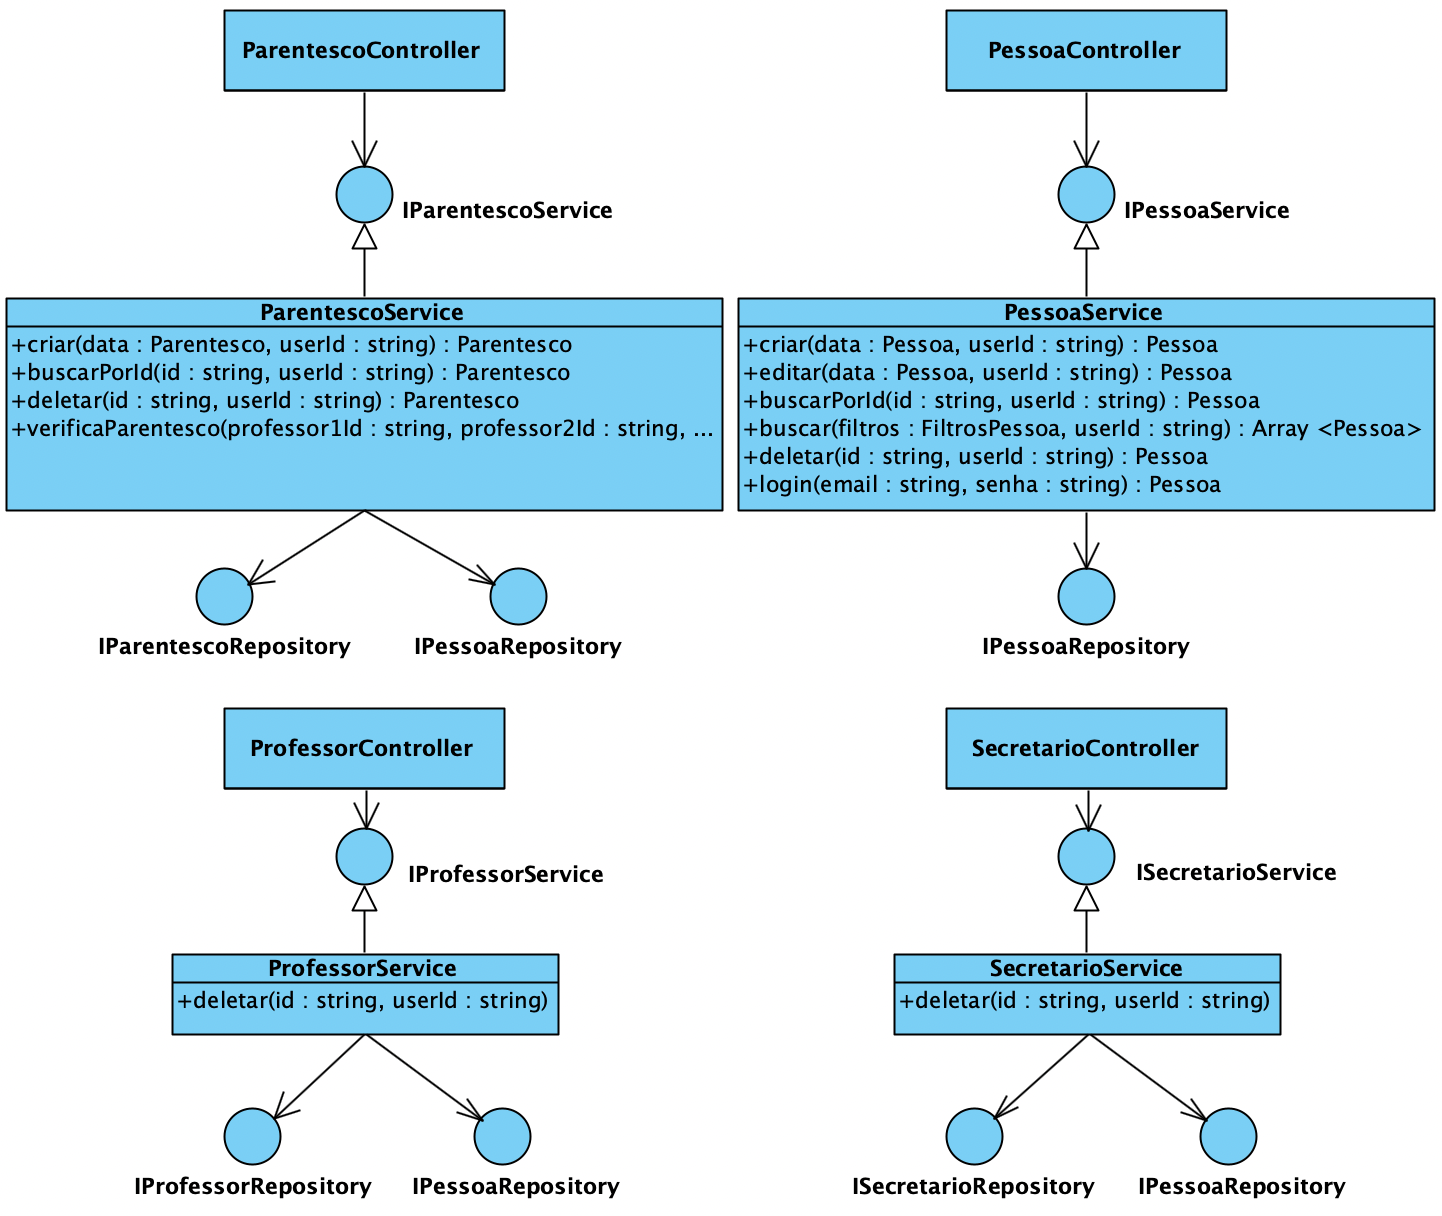
\includegraphics[width=0.9\textwidth]{figuras/fig-modelo-apl-2.png}
    \caption{Modelo de Aplicação do SCAP.}
    \label{fig-modelo-aplicacao-2}
\end{figure}

